\chapter{Saddle point approximation}
\label{cha:sp_approx}

%A semi-classical analysis of ATI which describes the formation of the
%ionization spectrum based on the interference of quantum paths is
%included in Sec.~\ref{sec:spa}. The direct ionization regime is
%considered independently in Sec.~\ref{sec:spa_direct}. The analysis
%presented in this chapter closely follows that
%of~\cite{KopoldOptComm2000}.

%\section{\label{sec:spa} Saddle point approximation}

For laser fields of sufficiently high intensity, the ATI spectrum can
be generated by implementing a saddle point
evaluation~\cite{LewensteinSPA_1994} of the multidimensional integral
for the transition amplitude obtained in the previous chapter. This
semi-classical approximation provides a deeper physical insight than
the expansion in Bessel functions from the improved Keldysh
approximation~\cite{Kopold_1997sfa} as it captures the essential
underlying physics. It also establishes a connection between ATI
calculations within the framework of the strong-field approximation
and the concept of quantum paths~\cite{KopoldOptComm2000}, which
represent space-time trajectories of the tunneling electrons. This
concept has its origins in the alternative formulation of quantum
mechanics introduced by Feynman in terms of path
integrals~\cite{RevModPhysFeynman}, where the probability amplitude of
a quantum mechanical process can be represented as a coherent
superposition of contributions from all possible spatio-temporal paths
that connect the initial and final state of the system.

The analysis presented in this chapter establishes the connection
between the quantum mechanical path integral formalism and the
improved Keldysh approximation discussed in Sec.~\ref{kopold_sfa}. The
transition amplitude that describes the ionization of an electron
under an external laser field is evaluated within the two frameworks,
that in which only direct electrons are considered as well as the case
that incorporates rescattering off the parent ion. Our study follows
those in Refs.~\cite{Kopold_1997sfa, KopoldOptComm2000}.

% see pra51 lewenstein

% mention that now that the matrix element for ionization has been
% introduced in the previous chapter, we are going to discuss an
% approximation to obtain the ionization spectrum where the integral
% over time is solved based on the stationary points method

\section{\label{sec:q_paths} Quantum-orbit formalism}
% formalism that derives the equations that describe the quantum paths
% and transition probability within the framework of spa

% describe the physics of the the three-step model where t, t' and k
% are introduced
Several quantum models have been introduced in the literature that
extend the scope of Keldysh approximation for strong laser-atom
interactions~\cite{LewensteinSPA_1994,Lewenstein_1995,Kopold_1997sfa}. These
models, which incorporate rescattering effects of the excited
electrons, have been valuable in unraveling the physical phenomena
behind the ATI plateau and its cutoff, an intrinsic feature of the
ionization spectrum. A quasi-classical analysis of this
generalization, based on the saddle point method and the path integral
formalism~\cite{KopoldOptComm2000,Becker_ellipticalSPA,LewScience2001},
has been particularly useful as it elucidates fundamental aspects of
the physics underlying strong-field ionization processes as well as
the formation of their spectra. This approach suggests that one
pictures the processes taking place in laser-atom interactions, such
as ATI and high-harmonic generation (HHG), in terms of electron
trajectories in phase space. These quantum trajectories follow
classical Newtonian dynamics, however, must take place in the complex
plane to account for tunneling. Consequently, they present non-zero
imaginary components which determine the probability of the
process. Their physical content is reflected in the electron dynamics
once it has been ionized at time $t'$, the electron may return to its
parent ion at a later time $t$ and rescatter after propagating with
momentum $\mathbf{k}$ in the continuum under the action of the
external field.

In the length gauge, the compact form of the Volkov state can be
expressed as
\begin{eqnarray}
\label{eq:volkov_Lgauge}
\begin{split}
|\psi_{\mathbf{p}}^{(V)}(t)\rangle & = &
|\mathbf{p} - e\mathbf{A}(t)\rangle e^{-i S_{\mathbf{p}}(t)},
\end{split}
\end{eqnarray}
where $|\mathbf{p} - e\mathbf{A}(t)\rangle$ represents a plane-wave
state and
$S_{\mathbf{p}}(t) = 1/2m \int\limits^{t} d\tau [\mathbf{p} -
e\mathbf{A}(\tau)]^{2}$
denotes the action of the system. Consequently, the Volkov
time-evolution operator can be written down in the form of an
expansion in terms of its Volkov states
\begin{eqnarray}
\label{eq:te_volkov}
\begin{split}
U^{(V)}(t,t') & = & \int d^{3}\mathbf{k}
|\psi_{\mathbf{k}}^{(V)}(t) \rangle
\langle \psi_{\mathbf{k}}^{(V)}(t')|.
\end{split}
\end{eqnarray}

Inserting the expansion~(\ref{eq:te_volkov}) into the matrix
element~(\ref{eq:mp_compact}) and given the time dependence of the
ground state wave function,
$|\psi_{0}(t) \rangle = \exp{(iE_{0}t)} | \psi_{0} \rangle$,
one may write~\cite{KopoldOptComm2000}
\begin{eqnarray}
\label{eq:me_action}
\begin{split}
M_{\mathbf{p}} = & \int\limits_{-\infty}\limits^{\infty} dt
\int\limits_{-\infty}\limits^{t} \int d^{3}\mathbf{k}
\ \langle \mathbf{p} - e\mathbf{A}(t) | V | \mathbf{k} - e\mathbf{A}(t) \rangle
\ \langle \mathbf{k} - e\mathbf{A}(t') | V | \psi_{0} \rangle \\
&
\times
\exp \left[i\left(-\frac{1}{2m} \int\limits_{t}\limits^{\infty}
d\tau [\mathbf{p} -e\mathbf{A}(\tau)]^{2} -
\frac{1}{2m} \int\limits_{t'}\limits^{t} d\tau [\mathbf{k} -e\mathbf{A}(\tau)]^{2} +
\int\limits_{-\infty}\limits^{t'} d\tau |E_{0}|
\right)
\right] \\
\sim &
\int\limits_{-\infty}\limits^{\infty} dt
\int\limits_{-\infty}\limits^{t} dt'
\int d^{3}\mathbf{k} \exp \left[ iS_{\mathbf{p}}(t, t', \mathbf{k}) \right]
m_{\mathbf{p}}(t, t', \mathbf{k}).
\end{split}
\end{eqnarray}
As one may notice, the action in the exponent, $S_{\mathbf{p}}(t, t',
\mathbf{k})$, contains three terms which correspond to the action of
the entire system after rescattering, between ionization and
rescattering and before ionization, respectively.

% point out the contrast with feynman's path integral
% p-57 chapter
It is revealing to point out the contrast of the ionization
amplitude~(\ref{eq:me_action}) obtained with the strong field
approximation with its analogous representation in terms of Feynman's
theory of path integral. The time evolution operator of the entire
system has the path integral representation
\begin{eqnarray}
\label{eq:te_path}
\begin{split}
U(\mathbf{r}t, \mathbf{r}'t') & = &
\int\limits_{(\mathbf{r}',t')\to(\mathbf{r},t)}
\mathcal{D}\left[ \mathbf{r}(\tau) \right] e^{i S(t, t')},
\end{split}
\end{eqnarray}
where $S(t, t') = \int\limits_{t'}\limits^{t} d\tau
\mathcal{L}[\mathbf{r}(\tau), \tau]$ is the action calculated along a
specific path by integrating the Lagrangian of the entire system along
that path, and the integral measure denoted by $\mathcal{D}\left[
  \mathbf{r}(\tau) \right]$ establishes a coherent sum over all
possible paths that connect $(\mathbf{r}t)$ and $(\mathbf{r}'t')$,
independently of whether or not the paths might be followed by the
actual system. This sum is, in fact, an infinite-dimensional
functional of integrals, and can be reduced, within the framework of
the strong-field approximation, to a sum over a few quantum orbits. By
implementing the strong-field approximation we have approximated the
exact action of the system at the various stages of the process:
before ionization, in between ionization and rescattering, and after
rescattering, as~(\ref{eq:me_action}) indicates, where the ionization
amplitude is computed through a sum over the exponential of the action
over a five-parameter set of paths, parametrized by the ionization
time $t'$, the rescattering time $t$ and the canonical momentum of the
orbit in between $\mathbf{k}$~\cite{KopoldOptComm2000}.

The five-dimensional set of paths over which the transition
amplitude~(\ref{eq:me_action}) is evaluated can be reduced further by
implementing a saddle point approximation of the
integral~\cite{KopoldOptComm2000}, in which a handful of relevant
paths remains to be considered. Since the quasi-classical actions in
Eq.~(\ref{eq:me_action}) are proportional to $I_{p}$, $U_{p}$, $p^{2}$
and $k^{2}$, which are large under intense laser fields, the factors
$\exp(-i S/\hbar)$ are rapidly oscillating and the integrals in the
transition amplitude can be approximated by the value of the
integrands at the stationary points, saddle points, of the
quasi-classical actions. The condition
\begin{eqnarray}
\label{eq:S_stationary}
\begin{split}
\frac{\partial S}{\partial q_{i}} & = & 0
\end{split}
\end{eqnarray}
where $q_{i}(i =1, \dots, 5)$ runs over the five variables $t$, $t'$
and $\mathbf{k}$, leads to the saddle-point
equations~\cite{Lewenstein_1995,KopoldOptComm2000}
\begin{eqnarray}
\label{eq:saddle_eqs}
\begin{split}
\left( \mathbf{k} - e\mathbf{A}(t') \right)^{2} = &
-2m|E_{0}| \\
\left( \mathbf{k} - e\mathbf{A}(t)\right)^{2} = &
\left( \mathbf{p} - e\mathbf{A}(t) \right)^{2} \\
(t - t') \mathbf{k} = & \int\limits_{t'}\limits^{t}
d\tau e\mathbf{A}(\tau).
\end{split}
\end{eqnarray}
The solutions
$(t_{S}(\mathrm{Re}\ t_{S} > \mathrm{Re}\ t'_{S}), t'_{S},
\mathbf{k}_{S})$,
are known as the stationary points of the quasicassical action of the
system, and define the quantum orbits over which the time integral
in~(\ref{eq:me_action}) needs to be carried out. From a physical
perspective, Eqs.~(\ref{eq:saddle_eqs}) ensure the energy conservation
at the time of tunneling, elastic scattering of the electron into its
final state when it returns, and that in fact the electron returns to
its parent ion, respectively. Since $|E_{0}| > 0$
in~(\ref{eq:saddle_eqs}), the condition of energy conservation at the
time of ionization cannot be satisfied for any real time $t'$. As a
consequence, the solutions $(t_{S}, t'_{S}, \mathbf{k}_{S})$ of the
saddle-point equations describe complex orbits which restrains a
straightforward visualization of the trajectories.

%p-56 chapter ATI
The matrix element~(\ref{eq:me_action}) can now be expressed in terms
of the saddle point solutions as~\cite{KopoldOptComm2000}
\begin{eqnarray}
\label{eq:Mp_final}
\begin{split}
M_{\mathbf{p}} \sim & \sum\limits_{i} \left( \frac{(2\pi i \hbar)^{5}}
{\mathrm{det} (\partial^{2}S / \partial q_{j} \partial q_{k})_{j,k = 1, \dots, 5}}
\right)^{1/2} \times \exp(i S(t_{S_{i}}, t'_{S_{i}}, \mathbf{k}_{S_{i}})),
\end{split}
\end{eqnarray}
where $q_{i}(i = 1,\dots,5)$ runs over the five variables $t_{S},
t_{S}'$ and $\mathbf{k}_{S}$. The sum~(\ref{eq:Mp_final}) involves a
reduced set of trajectories enough to determine the shape of the
ionization spectrum through their interferences, constructive or
destrutive.


\section{\label{sec:spa_results} Results}
% mention that we explore the quantum trajecotries that are relevant
% to the ATI spectrum

This section presents the results corresponding to a saddle-point
analysis of the probability amplitude to detect ATI electrons that
irradiate from a model-helium atom under a strong laser field of the
form~(\ref{eq:lp_field}). In order to obtain comparable results with a
saddle-point analysis to the quantum generalization of the
strong-field approximation presented in Chapter~\ref{cha:ati}, the
laser intensity and frequency were set to $I =
10^{15}\ \mathrm{W/cm^{2}}$ and $\hbar\omega = 0.0584\ \mathrm{a.u.}$,
respectively.

\subsection{\label{sec:spa_direct} Direct trajectories}

The probability amplitude for detecting an ATI electron that
propagates with momentum $\mathbf{p}$ in the continuum as a
consequence of the laser irradiation of an atom, which was originally
in its ground state, is studied in this section. The action that
describes the electron, bound to an atom with a binding energy
$E_{0}$, that is ionized at time $t_{0}$, without further interaction
with the parent ion, has the form
%
\begin{eqnarray}
  \label{eq:action_direct}
  \begin{split}
  S(t_{0}) & = &
-\frac{1}{2m}\int_{t_{0}}^{\infty}{d\tau [\mathbf{p} - e\mathbf{A}(\tau)]^{2}}
- \int_{-\infty}^{t_{0}}{d\tau E_{0}},
\end{split}
\end{eqnarray}
%
where $\mathbf{A}(t)$ represents the vector potential of the laser
field. As the main contribution to the transition
amplitude~(\ref{eq:Mp_final}) is given by the stationary points of the
action which satisfy the condition $dS_{\mathbf{p}} / dt_{0} = 0$, the
integral~(\ref{eq:Mp_final}) is evaluated by implementing a
saddle-point approximation~\cite{spa_1960}. This consists in expanding
the phase of the integrand, $\Phi(t) = (1/\eta) S(t) = (\omega /
U_{p}) S(t)$, in the vicinity of the points where the phase is
stationary. This results in determining the solutions of
%
\begin{eqnarray}
  \label{eq:stationary_points}
  \begin{split}
    \frac{\partial S}{\partial t_{0}} & = &
    \frac{1}{2m} (\mathbf{p} - e\mathbf{A}(t_{0}))^{2} + |E_{0}| = 0.
  \end{split}
\end{eqnarray}
%
Since the stationary points from Eq.~(\ref{eq:stationary_points}) have
a non-zero imaginary component, it is wise to deform the integral of
the action~(\ref{eq:Mp_final}) into the complex plane by implementing
the substitution $\omega t_{0} \to \rm{Re}(\omega t_{0}) +
i\rm{Im}(\omega t_{0})$. For a linearly polarized field of the
form~(\ref{eq:lp_field}), the saddle points can be determined
analytically and their real and imaginary components satisfy the
conditions
%
\begin{eqnarray}
  \label{eq:ReIm_eqs}
  \begin{split}
    \cos^{2}(\rm{Re}\ \omega t_{0s}) = & \frac{1}{2}
    \left( 1 + \gamma^{2} + \frac{E_{p}}{2U_{p}} \right)
    - \frac{1}{2}\sqrt{\left( \frac{E_{p}}{2U_{p}} \right)^{2}
    + (1 + \gamma^2)^2 + \frac{E_{p}}{U_{p}}(\gamma^2 - \cos 2\phi)}
    \\
    \cosh(\rm{Im}\ \omega t_{0s}) = & - \sqrt{\frac{E_{p}}{2U_{p}}}
    \frac{\cos\phi}{\cos(\rm{Re}\ \omega t_{0s})},
  \end{split}
\end{eqnarray}
%
where $m = -e = 1$ and $\phi$ is the angle between the momentum
$\mathbf{p}$ and the direction of polarization of the laser field,
$\hat{x}$. The electron energy, as it propagates in the continuum, is
indicated by $E_{p} = p^{2}/2m$. As Eqs.~(\ref{eq:ReIm_eqs}) indicate,
an individual value of $\mathbf{p}$ is associated with four
saddle-points $\omega t_{0s}$, $s = 1, \dots, 4$, which merge into one
another by complex conjugation. These complex roots are illustrated in
Figure~\ref{fig:sp_direct} for electron energies within the range $(0,
\dots, 6U_{p})$.

% include plot with the saddle-points for direct trajectories
\begin{figure}
  \centering
  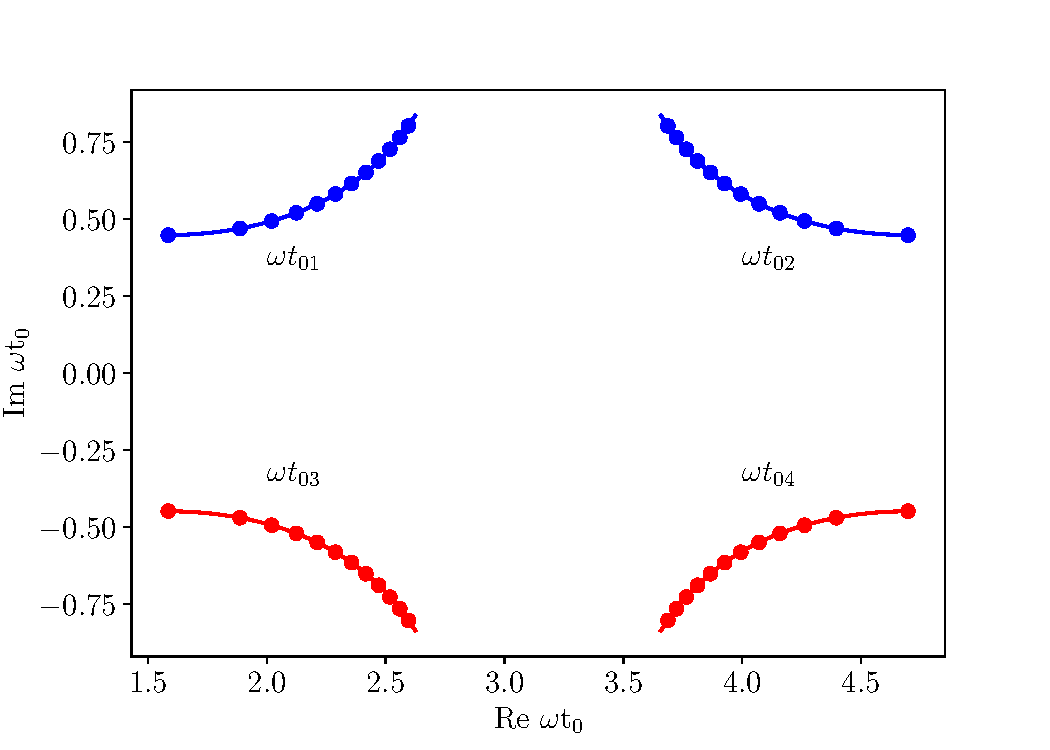
\includegraphics[width = 0.75\textwidth]{figures/ch_ATI_SPA/spDirectElectrons}
  \caption{Saddle points obtained from Eqs.~(\ref{eq:ReIm_eqs})
    associated with direct trajectories of electrons ionized by a
    linearly polarized field with laser intensity of
    $10^{15}\ \rm{W/cm^{2}}$ with $\hbar\omega = 1.58\ \rm{eV}$ for
    electron energies within $E_{p} < 6 U_{p}$.}
  \label{fig:sp_direct}
\end{figure}

In order to visualize the regions in phase-space where the action $S$
is stationary and, consequently, construct an integration path of
stationary phase over the saddle-points, it is convenient to carry out
the substitution $\tau \to \tau_{r} + i\tau_{i}$ in
Eq.~(\ref{eq:action_direct}). For a monochromatic laser
field~(\ref{eq:lp_field}), and assuming that the electron path is
parallel to the electric field of the laser, $\phi = 0$, the real and
imaginary components of the phase take the form~\cite{phd_Kopold}
%
\begin{eqnarray}
  \label{eq:phase_re_im}
  \begin{split}
    \rm{Im}(i\Phi(t)) & = & \omega t_{r} ( 1 + \frac{E_{p}}{U_{p}}
    + 2\gamma^{2} ) +
    \frac{1}{2} \sin 2\omega t_{r} \cosh 2\omega t_{i}
    + 2\sqrt{\frac{2E_{p}}{U_{p}}} \sin\omega t_{r} \cosh\omega t_{i}
    \\
    -\rm{Re}(i\Phi(t)) & = & \omega t_{i} (
    1 + \frac{E_{p}}{U_{p}} + 2\gamma^{2} )
    + \frac{1}{2} \cos 2\omega t_{r} \sinh 2\omega t_{i}
    + 2\sqrt{\frac{2E_{p}}{U_{p}}} \cos\omega t_{r} \sinh\omega t_{i}.
  \end{split}
\end{eqnarray}
% include contour plots for constant values of Im(\Phi) and
% integration path




\subsection{\label{sec:spa_resc} Trajectories with rescattering}








%%% Local Variables:
%%% mode: latex
%%% TeX-master: "thesis"
%%% End:
